\documentclass{beamer}
 
\usepackage[utf8]{inputenc}
\usepackage{siunitx}
\usetheme{CambridgeUS}
\useinnertheme{circles}

\usefonttheme[onlymath]{serif} 
 
%Information to be included in the title page:

\title{Seminar 3}
\subtitle{Classical mechanics}

\author{Will Barker\inst{1}\inst{2}}
\institute{
  \inst{1}%
    Cavendish Laboratory\\
    University of Cambridge\\
  \inst{2}%
    Kavli Institute for Cosmology\\
    University of Cambridge\\
}
\date{}
\logo{%
  \makebox[0.95\paperwidth]{%
    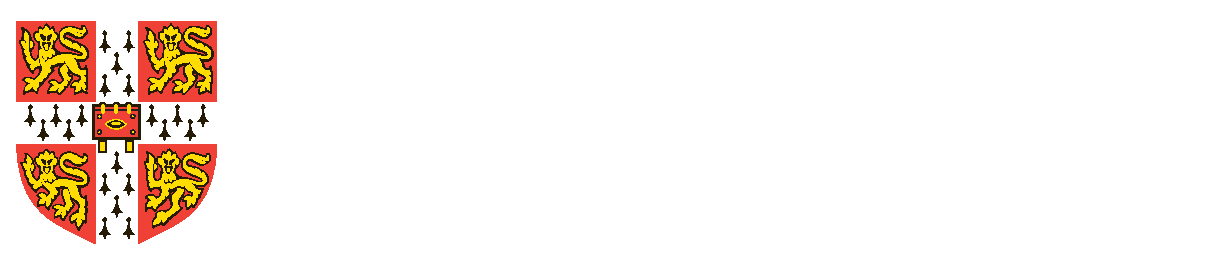
\includegraphics[height=0.7cm,keepaspectratio]{CU.eps}%
    \hfill%
    \includegraphics[height=0.7cm,keepaspectratio]{logo.png}%
  }%
}
 
 
 
\begin{document}
 
\frame{\titlepage}
 
\begin{frame}
  \frametitle{What is classical mechanics?}
  \begin{itemize}
    \item <1->Most importantly the \textbf{regime} $v\ll c$
    \item <2->Motion of \textbf{rigid bodies} or \textbf{point particles}
    \item <3->Can extend this to \textbf{continuous media}:
      \begin{itemize}
	\item <4->Fluid mechanics
	\item <5->Theory of elasticity
      \end{itemize}
  \end{itemize}
\end{frame}

\begin{frame}
  \center
  \frametitle{Quantities of interest}
  \begin{itemize}
    \item<1-> For a point particle, what do we mean by \textbf{coordinates}?
    \item<2-> What else can we define using \textbf{only} those coordinates?
    \item<3-> Any other properties of a point particle?
    \item<4-> In all:
      \begin{equation*}
	t, \quad \mathbf{x}, \quad \mathbf{v}, \quad \mathbf{a}, \quad m
      \end{equation*}
  \end{itemize}
\end{frame}

\begin{frame}
  \center
  \frametitle{Vectors}
  \begin{itemize}
    \item<1-> To make any progress whatever, we must be comfortable with the idea of \textbf{vectors}
    \item<2-> Position:
      \begin{equation*}
	\mathbf{x}=(x(t),y(t),z(t))=(x,y,z)	
      \end{equation*}
    \item<3-> Velocity:
      \begin{equation*}
	\mathbf{v}=\left(\frac{\mathrm{d}x(t)}{\mathrm{d}t},\frac{\mathrm{d}y(t)}{\mathrm{d}t},\frac{\mathrm{d}z(t)}{\mathrm{d}t}\right)=\left( \dot{x},\dot{y},\dot{z} \right)
      \end{equation*}
    \item<4-> Acceleration:
      \begin{equation*}
	\mathbf{a}=\left(\frac{\mathrm{d}^2x(t)}{\mathrm{d}t^2},\frac{\mathrm{d}^2y(t)}{\mathrm{d}t^2},\frac{\mathrm{d}^2z(t)}{\mathrm{d}t^2}\right)=\left( \ddot{x},\ddot{y},\ddot{z} \right)
      \end{equation*}
  \end{itemize}
\end{frame}

\begin{frame}
  \frametitle{Products of vectors}
  \begin{itemize}
    \item<1-> The \textbf{inner product} or \textbf{dot product} is the sum of the products of the components
      \begin{equation*}
	\mathbf{x}\cdot\dot{\mathbf{x}}=x\dot{x}+y\dot{y}+z\dot{z}
      \end{equation*}
    \item<2-> How about $\dot{\mathbf{x}}\cdot\ddot{\mathbf{x}}$?
    \item<3-> The inner product is also our means of talking about \textbf{distances}:
      \begin{equation*}
	\sqrt{\mathbf{x}\cdot\mathbf{x}}=\sqrt{x^2+y^2+z^2}	
      \end{equation*}
    \item<4-> Often we will need to take an inner product of a vector with itself:
      \begin{equation*}
	\mathbf{v}\cdot\mathbf{v}=v^2
      \end{equation*}
  \end{itemize}
\end{frame}

\begin{frame}
  \center
  \frametitle{Kinetic energy}
  \begin{itemize}
    \item<1-> \textbf{Kinetic energy} $T$ is just a number we associate with a moving particle of velocity $\mathbf{v}$ and mass $m$:
      \begin{equation*}
	T(\dot{\mathbf{x}})=\frac{1}{2}mv^2
      \end{equation*}
    \item<2-> As we mentioned in Seminar 1, this formula is \textbf{only} good for $v\ll c$
    \item<3-> As $v\to c$ nothing especially interesting happens, but if we use the \textbf{relativistic formula} we find that $T\to\infty$
  \end{itemize}
\end{frame}

\begin{frame}
  \center
  \frametitle{Potential energy}
  \begin{itemize}
    \item<1-> \textbf{Potential energy} $U$ is just a number we associate with a particle depending on its position in some \textbf{field}
    \item<2-> Simplest possible example, \textbf{voltage} or \textbf{electrical potential} $V(\mathbf{x})$ is a field, and a particle of mass $m$ has electrical charge $e$:
      \begin{equation*}
	U(\mathbf{x})=V(\mathbf{x})e
      \end{equation*}
    \item<3-> Any other potential fields we can think of?
  \end{itemize}
\end{frame}

\begin{frame}
  \center
  \frametitle{Force}
  \begin{itemize}
    \item<1-> Thus we have two (apparently meaningless) numbers that add to give total energy:
      \begin{equation*}
	\mathcal{  E}(\mathbf{x},\dot{\mathbf{x}})=U(\mathbf{x})+T(\dot{\mathbf{x}})
      \end{equation*}
    \item<2-> We are used to \textbf{forces} coming into play when we use Newton's laws
    \item<3-> This is dangerous, there is a far better definition which we need to understand:
      \begin{equation*}
	-\mathbf{F}(\mathbf{x})=\nabla U(\mathbf{x})
      \end{equation*}
  \end{itemize}
\end{frame}

\begin{frame}
  \frametitle{Grad}
  \begin{itemize}
    \item<1-> The upside-down triangle symbol $\nabla$ is known as \textbf{grad} or \textbf{gradient}
    \item<2-> Grad is a way of getting a vector from a scalar using differentiation:
      \begin{equation*}
	-\mathbf{F}(x,y,z)=\left(\frac{\partial U(x,y,x)}{\partial x},\frac{\partial U(x,y,z)}{\partial y},\frac{\partial U(x,y,z)}{\partial z}\right)
      \end{equation*}
    \item<3-> The Grad vector always points in the direction of \textbf{fastest change} of the field
  \end{itemize}
\end{frame}

\begin{frame}
  \frametitle{Energy conservation}
  \begin{itemize}
    \item<1-> What does \textbf{conservation} mean?
    \item<2-> When a particle moves through a potential field, the \textbf{total energy} is \textbf{conserved}:
      \begin{equation*}
	\dot{\mathcal{  E}}(\mathbf{x},\dot{\mathbf{x}})=0
      \end{equation*}
    \item<3-> Much easier to consider a \textbf{one-dimensional} example, where we only have the coordinate $x$
  \end{itemize}
\end{frame}

\begin{frame}
  \frametitle{Energy conservation}
  \begin{itemize}
    \item<1-> In the one-dimensional case:
      \begin{equation*}
      \mathcal{  E}(x,\dot{x})=U(x)+T(\dot{x}), \quad \dot{\mathcal{  E}}(x,\dot{x})=0
      \end{equation*}
    \item<2-> The function $U(x)$ could be \textbf{anything}, but what about the form of $T(\dot{x})$?
    \item<3-> Now what does the \textbf{second} equation tell us about the \textbf{first}?
    \item<4-> We should get:
      \begin{equation*}
	\dot{x}\frac{\mathrm{d}U(x)}{\mathrm{d}x}+m\dot{x}\ddot{x}=0
      \end{equation*}
  \end{itemize}
\end{frame}

\begin{frame}
  \frametitle{Energy conservation}
  \begin{itemize}
    \item<1-> So \textbf{conservation of energy tells us}:
      \begin{equation*}
	\dot{x}\frac{\mathrm{d}U(x)}{\mathrm{d}x}+m\dot{x}\ddot{x}=0
      \end{equation*}
    \item<2-> We can tidy this up a bit with $\dot{x}=v$, $\ddot{x}=a$ and $\frac{\mathrm{d}U(x)}{\mathrm{d}x}=-F(x)$:
      \begin{equation*}
	-vF(x)+mva=0
      \end{equation*}
    \item<3-> But $v$ could be anything, so we can divide it away:
      \begin{equation*}
	F(x)=ma
      \end{equation*}
  \end{itemize}
\end{frame}

\begin{frame}
  \frametitle{Newton's laws}
  \begin{itemize}
    \item<1-> So we've just used \textbf{energy conservation} to derive \textbf{Newton's 2nd law}:
      \begin{equation*}
	F(x)=ma
      \end{equation*}
    \item<2-> What is the \textbf{1st} law?
    \item<3-> What if we set $F(x)=0$?
  \end{itemize}
\end{frame}

\begin{frame}
  \frametitle{Newton's laws}
  \begin{itemize}
    \item<1-> This was just the case in \textbf{one dimension}, the energy conservation equation for all \textbf{three} space dimensions has to be written in textbf{vector form}:
      \begin{equation*}
	\dot{\mathbf{x}}\cdot\nabla U(\mathbf{x})+m\dot{\mathbf{x}}\cdot\ddot{\mathbf{x}}=0
      \end{equation*}
    \item<2-> And again we can write these vectors with more sensible names:
      \begin{equation*}
	\mathbf{v}\cdot\left( -\mathbf{F}(\mathbf{x})+m\mathbf{a} \right)=0
      \end{equation*}
    \item<3-> And since $\mathbf{v}$ is completely general:
      \begin{equation*}
	\mathbf{F}(\mathbf{x})=m\mathbf{a}
      \end{equation*}
  \end{itemize}
\end{frame}

\begin{frame}
  \frametitle{Newton's laws}
  \begin{itemize}
    \item<1-> So we understand now that Newton's \textbf{1st} law is just a special case of Newton's \textbf{2nd} law
    \item<2-> What about Newton's \textbf{3rd} law?
    \item<3-> This is far more complicated, and requires \textbf{two or more} particles:
      \begin{itemize}
	\item<4-> The \textbf{potential} field (e.g. $V(\mathbf{x})$) usually comes from a \textbf{second} particle
	\item<5-> The \textbf{3rd} law guarantees \textbf{energy conservation} for \textbf{multiple particles} along with \textbf{momentum conservation}
	\item<6-> When we consider all particles and potentials, we are talking about a \textbf{system} in which total \textbf{energy} and total \textbf{momentum} are conserved
      \end{itemize}
  \end{itemize}
\end{frame}

\begin{frame}
  \frametitle{Some deep principles}
  \begin{itemize}
    \item<1-> There is a vary powerful formalism that describes all of \textbf{classical mechanics}, \textbf{quantum mechanics} and \textbf{general relativity}, known as the \textbf{Lagrangian formalism} or \textbf{Hamilton's principle}:
      \begin{itemize}
	\item<2-> \textbf{Energy conservation} happens because the laws of physics are the same at all points in \textbf{time}
	\item<3-> \textbf{Momentum conservation} happens because the laws of physics are the same at all points in \textbf{space}
      \end{itemize}
    \item<4-> Energy is a \textbf{scalar} (one \textbf{time} dimension), momentum is a \textbf{vector} (three \textbf{space} dimensions)
    \item<5-> The fancy word for this is \textbf{Noether symmetry}
  \end{itemize}
\end{frame}

\begin{frame}
  \center
  \frametitle{Some deep principles}
  \includegraphics[height=5cm]{noether.jpg}
\end{frame}

\begin{frame}
  \frametitle{The pendulum}
  \begin{itemize}
    \item<1-> Mostly in school the conservation laws are applied to \textbf{particles colliding} or, even worse, \textbf{trolleys} colliding
    \item<2-> This is the most \textbf{boring} example in the universe
    \item<3-> The \textbf{pendulum} is far more interesting, but since it is effectively \textbf{one} particle (the mass on the end) we can't build a picture of \textbf{momentum conservation}
    \item<4-> What is the potential energy?
  \end{itemize}
\end{frame}

\begin{frame}
  \frametitle{The pendulum}
  \begin{itemize}
    \item<1-> The pendulum is an example of a \textbf{constrained} system, the particle is confined to move only in a circle of radius $l$, and the coordinate that defines its position is $\theta$
    \item<2-> We can think of $\theta$ playing the r\^ole of $x$ in the \textbf{one dimensional} case of Newton's 2nd law
    \item<3-> The \textbf{velocity} has the magnitude:
      \begin{equation*}
	v=l\dot{\theta}
      \end{equation*}
    \item<4-> The \textbf{acceleration} has the magnitude:
      \begin{equation*}
	a=l\ddot{\theta}
      \end{equation*}
  \end{itemize}
\end{frame}

\begin{frame}
  \frametitle{The pendulum}
  \begin{itemize}
    \item<1-> Because the particle is constrained, the $F(\theta)$ that will enter into Newton's 2nd law has to be the \textbf{component} of $\mathbf{F}(\mathbf{x})$ that points along the path of the particle
    \item<2-> \textbf{Find the formula for} $F(\theta)$
  \end{itemize}
\end{frame}

\begin{frame}
  \frametitle{The pendulum}
  \begin{itemize}
    \item<1-> We should have $F(\theta)=-mg\sin(\theta)$
    \item<2-> This means for Newton's 2nd law:
      \begin{equation*}
	F(\theta)=ma\implies -mg\sin(\theta)=ml\ddot{\theta}
      \end{equation*}
    \item<3-> Dividing through by $m$ (because $m\neq 0$) gives:
      \begin{equation*}
	\ddot{\theta}=-\frac{g}{l}\sin{\theta}
      \end{equation*}
  \end{itemize}
\end{frame}

\begin{frame}
  \frametitle{The pendulum}
  \begin{itemize}
    \item<1-> So now we have a \textbf{differential equation} describing the motion of a pendulum:
      \begin{equation*}
	\ddot{\theta}=-\frac{g}{l}\sin{\theta}
      \end{equation*}
    \item<2-> It looks very simple, but actually it is very difficult to solve (requires \textbf{elliptic integrals})
    \item<3-> To make it super easy we use the \textbf{small angle approximation} $\theta\ll 1$:
      \begin{equation*}
	\sin(\theta)=\theta-\frac{1}{6}\theta^3+\frac{1}{120}\theta^5-\cdots
      \end{equation*}
  \end{itemize}
\end{frame}

\begin{frame}
  \frametitle{The pendulum}
  \begin{itemize}
    \item<1-> So now we are approximating $\sin(\theta)\approx\theta$, the differential equation becomes:
      \begin{equation*}
	\ddot{\theta}=-\frac{g}{l}\theta
      \end{equation*}
    \item<2-> This looks even easier than before, \textbf{solve it} using what we learned in Seminar 1, and assuming $\frac{g}{l}=1$:
      \begin{gather*}
	f(t)=e^t\implies \dot{f}(t)=e^t, \quad \ddot{f}(t)=e^t\\
	f(t)=\cosh(t)\implies \dot{f}(t)=\sinh(t), \quad \ddot{f}(t)=\cosh(t)\\
	f(t)=\sinh(t)\implies \dot{f}(t)=\cosh(t), \quad \ddot{f}(t)=\sinh(t)\\
	f(t)=\cos(t)\implies \dot{f}(t)=-\sin(t), \quad \ddot{f}(t)=-\cos(t)\\
	f(t)=\sin(t)\implies \dot{f}(t)=\cos(t), \quad \ddot{f}(t)=-\sin(t)\\
      \end{gather*}
  \end{itemize}
\end{frame}


\begin{frame}
  \center
  \frametitle{Astrophysical phenomena}
  \includegraphics[height=5cm]{big_bang.jpg}
\end{frame}

\end{document}


